\section{Dynamiczne WWW i ASP.NET}

\subsection{Dlaczego potrzebujemy dynamicznego WWW}

Gwałtowny rozwój sieci i coraz szerszy dostęp do niej sprawiają, że równie szybko rozwijają się techologie
sieciowe. Zwykły protokół HTML, choć w wielu przypadkach sprawdza się doskonale, w wielu innych okazuje się
niewystarczający. To czego potrzebują programiści, to możliwość tworzenia {\em dynamicznych} stron
Internetowych, przy czym przez {\em dynamiczny} nie oznacza tu "animowany, żywy", tylko dostosowany do
profilu konkretnego użytkownika i umożliwiający komunikację w dwie strony. 

Dynamicznie budowana zawartość stron WWW najczęściej związana jest jakoś z dużymi zbiorami informacji.
Wyobraźmy sobie sieciową encyklopedię, w której istnieją setki tysięcy
możliwych haseł, czy system ewidencji z milionami rekordów. Nietrudno zauważyć, że sam HTML jest zbyt
ubogi, aby wspomagać realizację takich przedsięwzięć (chyba, że ktoś wie jak przygotować milion stron 
w HTML i zbudować dla nich sensowne indeksy).

\subsection{Przegląd technologii dynamicznego WWW}

\subsubsection{Common Gateway Interface}

CGI jest jedną z pierwszych technologii, umożliwiających tworzenie dynamicznych stron WWW. 
Pomysł CGI polega na tym, że serwer Internetowy uruchamia zwykły program wykonywalny (nazywany
{\bf skryptem CGI}) i wyniki działania tego programu przekazuje klientowi. Jedna z zalet CGI
polega na tym, że skrypty mogą być napisane w dowolnym języku, w którym da się napisać konsolowy
program, który zapisuje i odczytuje dane ze standardowych strumieni wejścia/wyjścia.

Najprostszy skrypt CGI, napisany w języku C mógłby wyglądać tak:

\begin{scriptsize}
\begin{verbatim}
#include <stdio.h>

int main( int argc, char** argv )
{
  printf( "HTTP/1.0 200 OK\r\nContent-type: text/html\r\n\r\n" );
  printf( "<HTML>\r\n<HEAD>" );
  printf( "<TITLE>Witam w CGI</TITLE></HEAD>\r\n" );
  printf( "<BODY>Pierwszy skrypt w CGI</BODY>\r\n" );
  printf( "</HTML>" );

  return 0;
}
\end{verbatim}
\end{scriptsize}

Z racji prostej idei, CGI jest bardzo popularne. Z CGI związane są jednak duże problemy z wydajnością.
Po pierwsze, kiedy skrypt jest wykonywany na serwerze, jest traktowany jak każdy inny proces w systemie,
a co za tym idzie musi być inicjowany jak każdy inny proces. Z punktu widzenia systemu operacyjnego, inicjowanie
nowego procesu jest dość czasochłonne. Po drugie, każdy nowy skrypt CGI zajmuje pamięć wprost proporcjonalną do
swojej wielkości. Przy stu użytkownikach korzystających jednocześnie z serwera jest to jeszcze możliwe.
Przy kilku tysiącach jednocześnie uruchomionych procesów zasoby nawet bardzo rozbudowanego serwera najprawdopodobniej
ulegną wyczerpaniu i cały system zawali się.

\subsubsection{Internet Server Application Programming Interface}

Aby pokonać problemy związane z wydajnością CGI, Microsoft zaprojektował alternatywną technologię
dynamicznego WWW, nazwaną Internet Server Application Programming Interface (ISAPI). Główny pomysł
polegał na tym, że skrypty ISAPI są bibliotekami (DLL) a nie modułami wykonywalnymi, dzięki czemu
kod skryptu ładowany jest do pamięci tylko raz.

Istnieją dwa rodzaje bibliotek ISAPI: {\bf rozszerzenia ISAPI}, które spełniają identyczną funkcję
jak skrypty CGI oraz {\bf filtry ISAPI}, które reagują na pewne zdarzenia związane z obsługą stron
przez serwer.

Mimo, że technologia ISAPI jest zdecydowanie wydajniejsza od CGI, nie jest pozbawiona wad. Po pierwsze,
napisanie poprawnej biblioteki ISAPI wymaga zdecydowanie więcej wiedzy niż napisanie skryptu CGI.
Po drugie, jeśli biblioteka ISAPI trafi już na serwer Internetowy, to nie ma łatwego sposobu na
zastąpienie jej nowszą wersją, ponieważ system operacyjny zabroni dostępu do biblioteki, która wedle jego
rozeznania będzie cały czas używana. Wymiana biblioteki wymaga więc zatrzymania usługi serwera
Inernetowego na serwerze sieciowym.

\subsubsection{ASP}

Następcą ISAPI jest technologia {\bf Active Server Pages}, która, o dziwo, jest zaimplementowana jako
rozszerzenie ISAPI. W przypadku ASP nie ma jednak konieczności pisania własnych bibliotek DLL. Zamiast
tego tworzy się zwykłą stronę HTML, zaś wewnątrz jej kodu można umieszczać dowolne instrukcje
kodu języka skryptowego VBScript. ASP sam dba o interpretowanie kodu VBScript i odsyła do klienta
wyniki tej operacji.

Oto przykład bardzo prostej strony ASP:

\begin{scriptsize}
\begin{verbatim}
<% Option Explicit %>
<HTML>
<HEAD><TITLE>Witam w ASP</TITLE></HEAD>
<BODY>
<%
Dim n
For n = 1 to 5
  Response.Write( "<FONT size=" & n )
  Response.Write( ">Witam w ASP</FONT><br>" & vbCrLf )
Next
%>
</BODY>
</HTML>
\end{verbatim}
\end{scriptsize}

Projektując strony ASP można korzystać z całej siły VBScript. Ale to właśnie siła VBScript ta okazuje 
się być największą słabością ASP - VBScript, jak przystało na język skryptowy, 
jest bardzo słabo otypowany. Co więcej 
- strony są interpretowane dynamicznie. Oba te fakty oznaczają, że bardzo łatwo popełniać błędy
w skryptach, które jeśli się pojawią, to wykrywane są dopiero wtedy, kiedy natrafi na nie pierwszy
użytkownik.

\subsection{Czym jest ASP.NET}

ASP.NET jest naturalnym rozszerzeniem ASP, które integruje technologię ASP z platformą .NET.
Dzięki ASP.NET możliwe jest używanie praktycznie dowolnego języka platformy .NET do tworzenia
dynamicznej zawartości stron WWW. W chwili obecnej jednak ASP.NET (podobnie jak ASP) działa
jedynie na serwerze WWW wbudowanym w systemy Windows począwszy od wersji 2000. Serwer ten
to {\bf Microsoft Internet Information Services} (IIS).

\subsection{Pierwszy przykład w ASP.NET}

Najprostszy przykład dynamicznej strony ASP.NET ukazuje jednocześnie, że ASP.NET umożliwia
użycie C\# jako języka skryptowego\footnote{Kod wewnątrz strony może być napisany w C\# lub VB.NET. 
Tylko kod umieszczony w obiektowych bibliotekach DLL, będących dodatkowymi elementami dynamicznej strony, 
może zawierać skompilowany kod napisany w dowolnym języku .NET}. Przy próbie uruchomienia kod strony będzie
prekompilowany, a błędy będą statycznie raportowane użytkownikowi. 

Druga ważna różnica między ASP a ASP.NET to brak możliwości bezpośredniego odwołania się
do zawartości tekstu strony HTML. W ASP bardzo często używa się metody {\bf Response.Write}, aby
umieścić tekst wewnątrz strony ASP. W ASP.NET można jedynie odwoływać się do umieszczonych na stronie
obiektów WWW lub kontrolek ASP.NET. W poniższym przykładzie odwołujemy się do obiektu WWW typu
{\bf SPAN}. Dostęp do obiektu możliwy jest dzięki odwołaniu się do jego nazwy (w przykładzie
obiekt typu SPAN nazywa się {\bf Message}).

\begin{scriptsize}
\begin{verbatim}
<%@ Page Language="C#" %>
<HTML>
<HEAD><TITLE>Witam w ASP.NET</TITLE></HEAD>
<BODY>

<%
int    i;
string s = string.Empty;

for ( i=1; i<=5; i++ )
{
  s = s+String.Format( 
    "<FONT size={0}>Witam w ASP.NET</FONT><br>", i );
}
Message.InnerHtml = s;
%>

<SPAN id="Message" runat=server/>

</BODY>
</HTML>
\end{verbatim}
\end{scriptsize}

\subsection{Łączenie stron ASP.NET z dowolnym kodem}

Jedną z najciekawszych możliwości ASP.NET jest łączenie kodu strony z dowolnym kodem, kompilowanym
przy pomocy dowolnego kompilatora platformy .NET. 

Napiszmy najpierw kod prostej klasy:

\begin{scriptsize}
\begin{verbatim}
using System;

namespace NExample
{
  public class COsoba
  {
     public string Imie;
     public string Nazwisko;

     public COsoba( string Imie, string Nazwisko )
     {
       this.Imie     = Imie; 
       this.Nazwisko = Nazwisko;
     }

     public override string ToString()
     {
       return String.Format( "{0} {1}", Nazwisko, Imie );
     }
  }
}
\end{verbatim}
\end{scriptsize}

i skompilujmy go do postaci biblioteki:

\begin{scriptsize}
\begin{verbatim}
C:\Example>csc.exe /target:library CExample.cs
\end{verbatim}
\end{scriptsize}

Aby tak utworzona biblioteka mogła być wykorzystana w kodzie strony, plik DLL musi być umieszczony
w podkatalogu {\bf bin} katalogu wirtualnego IIS. Katalog taki może być utworzony ręcznie i nie musi
mieć ustawionych żadnych specjalnych praw dostępu.
Aby moć korzystać z przygotowanej klasy, w kodzie strony należy tylko dodać odwołanie do odpowiedniej
przestrzeni nazw. 

\begin{scriptsize}
\begin{verbatim}
<%@ Page Language="C#" %>
<%@ import Namespace="NExample" %>
<HTML>
<HEAD><TITLE>Witam w ASP.NET</TITLE></HEAD>
<BODY>

<%
COsoba osoba = new COsoba( "Jan", "Kowalski" );
int    i;
string s = string.Empty;

for ( i=1; i<=5; i++ )
{
  s = s+String.Format( 
    "<FONT size={0}>{1}</FONT><br>", i, osoba );
}
Message.InnerHtml = s;
%>

<SPAN id="Message" runat=server/>

</BODY>
</HTML>
\end{verbatim}
\end{scriptsize}

Użytkownik, który ogląda naszą stronę w przeglądarce i próbuje podglądnąć źródło strony, widzi
oczywiście tylko efekt końcowy:

\begin{figure}
\begin{center}
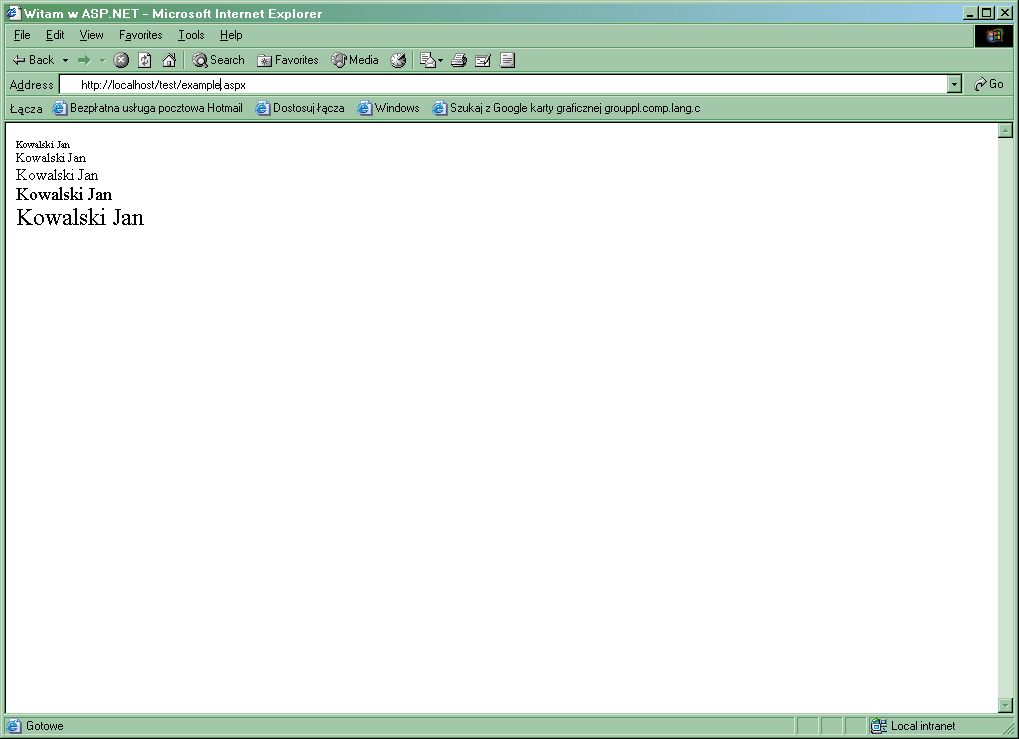
\includegraphics[width=0.50\textwidth]{./pic/asp01}
\caption{Efekt końcowy w przeglądarce}
\end{center}
\end{figure}

\begin{scriptsize}
\begin{verbatim}
<HTML>
<HEAD><TITLE>Witam w ASP.NET</TITLE></HEAD>
<BODY>

<SPAN id="Message">
<FONT size=1>Kowalski Jan</FONT><br>
<FONT size=2>Kowalski Jan</FONT><br>
<FONT size=3>Kowalski Jan</FONT><br>
<FONT size=4>Kowalski Jan</FONT><br>
<FONT size=5>Kowalski Jan</FONT><br></SPAN>

</BODY>
</HTML>
\end{verbatim}
\end{scriptsize}

\subsection{Kontrolki ASP.NET}

Kod strony ASP.NET może oczywiście zawierać komponenty WWW, takie, jakie można umieszczać na
zwykłych stronach HTML. Oprócz tego można jednak korzystać z całej gamy komponentów właściwych dla
ASP.NET. Komponenty te są obiektami pochodzącymi z biblioteki {\bf System.Web.UI.WebControls}.
Programista może oczywiście sam tworzyć własne komponenty wizualne, dziedzicząc z klasy
{\bf System.Web.UI.UserControl}.

Zbiór zdarzeń, jakie udostępniają komponenty ASP.NET różni się od zdarzeń komponentów Windows.Forms.
Jest to dość oczywiste - zachowanie się komponentów w systemie operacyjnym podlega innym regułom
niż zachowanie się komponentów w przeglądarce Internetowej.

Przykładowy skrypt tworzy dwa komponenty ASP.NET, etykietę i przycisk. Zauważmy, że definicje 
komponentów są częścią strony i wyróżniają się jedynie specjalnymi atrybutami. Wewnątrz definicji 
przycisku określono funkcję reagującą na przyciśnięcie przycisku. Funkcję tę umieszczono wewnątrz
specjalnej sekcji strony, oznaczonej tagami {\bf script}.

\begin{scriptsize}
\begin{verbatim}
<%@ Page Language="C#" %>

<script runat="server">
    void Przycisk_Click(Object sender, EventArgs e) {
        Label1.Text = "Witam w ASP.NET";
    }
</script>

<html>
<head>
</head>
<body>
  <form runat="server">
  <center>
    <asp:Label id="Label1" runat="server" 
               Width="193px">Etykieta</asp:Label>
    <br />
    <asp:Button id="Przycisk" onclick="Przycisk_Click" 
                runat="server" Text="Twórz dane osobowe" 
		Width="192px"></asp:Button>
  </center>
  </form>
</body>
</html>
\end{verbatim}
\end{scriptsize}

Wśród komponentów ASP.NET znajduje się m.in. kilka rodzajów siatek, przycisków, kalendarze. Wśród nich 
jest na przykład {\bf DataGrid}, który może być inicjowany w standardowy sposób (patrz rozdział 
\ref{DataGrid}, strona \pageref{DataGrid}).

\subsection{Inne przykłady ASP.NET}

\subsubsection{Identyfikacja klienta}

Wewnątrz kodu strony można odwoływać się do wszystkich składowych obiektu {\bf Page}, identyfikującego
bieżącą stronę. Wśród nich przydatne są propercje {\bf Request} określająca parametry strony inicjującej
połączenie oraz {\bf Response} określająca parametry odpowiedzi serwera.

Propercja {\bf Request} może być wykorzystana na przykład do identyfikacji systemu operacyjnego
i przeglądarki, której używa klient.

\begin{scriptsize}
\begin{verbatim}
<%@ Page Language="C#" %>
<HTML>
<HEAD><TITLE>Witam w ASP.NET</TITLE></HEAD>
<BODY>

<%
Message.InnerHtml = String.Format( "Browser: {0}, platform {1}", 
                     Request.Browser.Browser, 
		     Request.Browser.Platform );
%>

<SPAN id="Message" runat=server/>

</BODY>
</HTML>
\end{verbatim}
\end{scriptsize}

\subsubsection{Licznik odwiedzin strony}

Przygotowanie licznika odwiedzin strony jest jedym z podstawowych zadań dynamicznego WWW. W ASP.NET sytuacja jest
o tyle wygodna, że w kodzie skryptów używamy dobrze znanych bibliotek .NET.

Wartość licznika odwiedzin będzie zapisywana w pliku {\tt counter.txt} w folderze strony WWW.
Jak jednak zabiezpieczyć się przed zwiększaniem tego licznika przy częstym odświeżaniu strony
przez Internautę? Możemy skorzystać z {\em ciasteczek}, czyli informacji umieszczanych po stronie
klienta, które pozwalają identyfikować go przy kolejnych odwiedzinach naszej strony. W poniższym
przykładzie ciasteczko zostanie unieważnione po 2 minutach od pierwszego wejścia na stronę WWW.

\begin{scriptsize}
\begin{verbatim}
<%@ Page Language="C#"%> 
<%@ import Namespace="System.IO" %> 
<%@ import Namespace="System.Drawing" %> 
<%@ import Namespace="System.Drawing.Imaging" %> 
<%@ import Namespace="System.Drawing.Drawing2D" %> 

<script runat="server" language="C#">

string getCounter()
{ 
  string CookieID = "OldVisitor";

  // czytaj wartosc licznika
  string FilePath = Server.MapPath("\\") + "counter.txt"; 
  StreamReader sr = File.OpenText(FilePath); 
  string counter  = sr.ReadLine().ToString(); 
  sr.Close(); 

  // ciasteczko - czy to stary gość?
  HttpCookie Cookie; 
  Cookie = Request.Cookies[CookieID]; 

  // tak, inkrementuj licznik
  if(Cookie==null) 
  { 
    int counterInt = Convert.ToInt32(counter); 
    counterInt++; 
    counter = Convert.ToString(counterInt); 

    FileStream   fs = new FileStream(FilePath, FileMode.Open, FileAccess.Write); 
    StreamWriter sw = new StreamWriter(fs); 
    sw.WriteLine(counter); 
    sw.Close(); 
    fs.Close(); 

    Cookie         = new HttpCookie( CookieID, "true" ); 
    Cookie.Expires = DateTime.Now.AddSeconds( 120 ); 
    Response.AppendCookie( Cookie ); 
  } 

  return counter; 
} 

</script> 

<HTML>
<HEAD><TITLE>Przykładowy licznik w ASP.NET</TITLE></HEAD>
<BODY>

<% MyCounter.InnerHtml = getCounter(); %>

<center>
Gość numer: <SPAN id="MyCounter" runat=server/>
<asp:Image id="MyCounterImage"/>
</center>

</BODY>
</HTML>
\end{verbatim}
\end{scriptsize}

Spróbujmy rozwinąć trochę ten przykład, tak aby licznik odwiedzin był umieszczony na stronie
w postaci nie tekstu, ale dynamicznie budowanego obrazka.

W pierwszej chwili może wydać się to trudne, ale na szczęście w kodzie strony istnieje możliwość
zapisania wyglądu strony w postaci strumienia danych. 

\begin{scriptsize}
\begin{verbatim}
// Plik: c.aspx
<%@ Page Language="C#"%> 
<%@ import Namespace="System.IO" %> 
<%@ import Namespace="System.Drawing" %> 
<%@ import Namespace="System.Drawing.Imaging" %> 
<%@ import Namespace="System.Drawing.Drawing2D" %> 

<script runat="server" language="C#">

string getCounter()
{ 
  // ... to samo co poprzednio
} 

void drawCounter() 
{ 
  int height = 40; 
  int width  = 120; 

  Bitmap bmp = new Bitmap( width, height ); 
  Graphics g = Graphics.FromImage(bmp); 

  string currentCounter = getCounter(); 
  Font      counterFont = new Font( "Arial", 24, FontStyle.Bold ); 
  SizeF           sizeF = g.MeasureString( currentCounter, counterFont ); 

  g.FillRectangle( Brushes.Black, 0, 0, width, height ); 
  g.DrawString( currentCounter, counterFont, 
                Brushes.White, (bmp.Width-sizeF.Width)/2, 3 ); 

  bmp.Save(Response.OutputStream, ImageFormat.Jpeg); 

  g.Dispose(); 
  bmp.Dispose(); 
} 

private void Page_Load(object sender, System.EventArgs e)
{
  drawCounter();		
}
</script> 
\end{verbatim}
\end{scriptsize}

\begin{figure}
\begin{center}
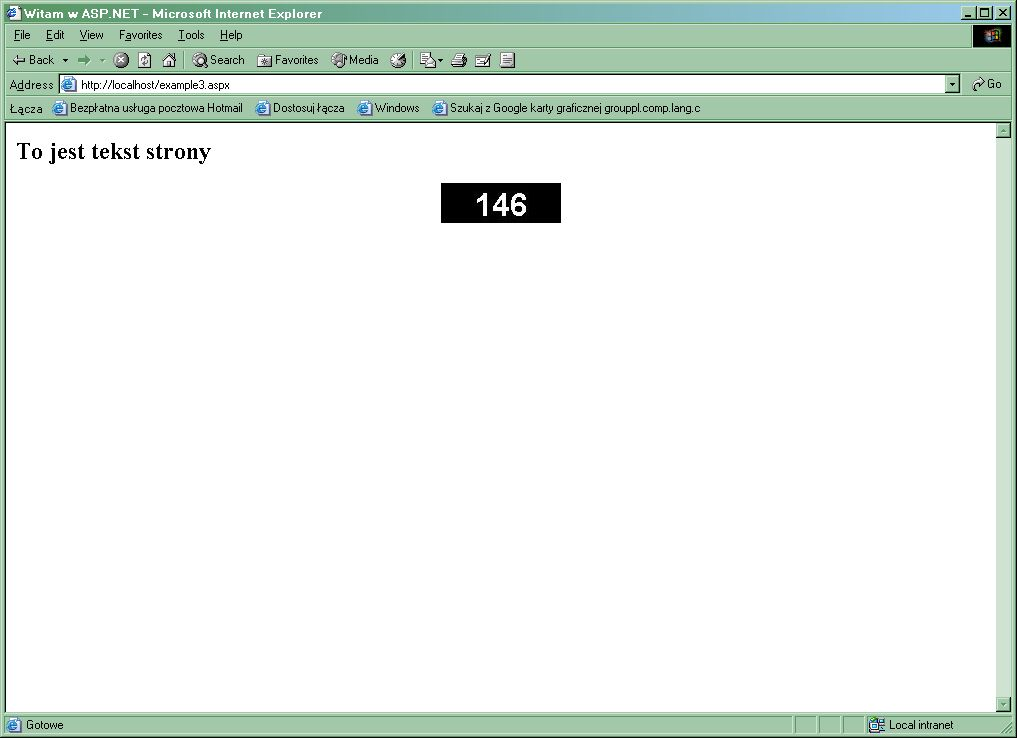
\includegraphics[width=0.75\textwidth]{./pic/asp03}
\caption{Dynamiczny licznik odwiedzin strony w ASP.NET}
\end{center}
\end{figure}

Tak przygotowana strona pokazuje wartość licznika w postaci obrazka. Problem polega tylko na tym, że
zapisanie strumienia danych do zawartości strony ({\bf bmp.Save(Response.OutputStream,...})
powoduje, że strona nie będzie zawierać żadnych innych obiektów. To nie szkodzi! Z licznika
skorzystamy w kodzie każdej kolejnej strony, dynamicznie dołączając go jako obrazek:

\begin{scriptsize}
\begin{verbatim}
<%@ Page Language="C#" %>
<HTML>
<HEAD><TITLE>Witam w ASP.NET</TITLE></HEAD>
<BODY>

<h2>To jest tekst strony</h2>

<center>
<img src="c.aspx"/>
</center>

</BODY>
</HTML>
\end{verbatim}
\end{scriptsize}

\subsection{Narzędzia wspomagające projektowanie stron ASP.NET}

\subsubsection{Visual Studio .NET}

Visual Studio .NET znakomicie radzi sobie ze wspomaganiem projektowania stron ASP.NET. Z poziomu
środowiska, tworząc nowy projekt, można nawet utworzyć katalog wirtulany na serwerze IIS. 

Podczas pracy nad projektem Visual Studio .NET stosuje nieco inną konwencję od przedstawionej
w dotychczasowych przykładach - warstwa prezentacyjna (układ komponentów) znajduje się w osobnym pliku
niż kod obsługi zdarzeń komponentów. 

\subsubsection{ASP.NET WebMatrix}

Microsoft ASP.NET WebMatrix jest darmowym narzędziem, wspierającym projektowanie stron ASP.NET. 
WebMatrix ma wizualny edytor stron, edytor kodu, palety narzędziowe. Edytor pozwala na przypisywanie zdarzeń
komponentom.

WebMatrix można pobrać ze strony {\bf http://www.asp.net}.

\begin{figure}
\begin{center}
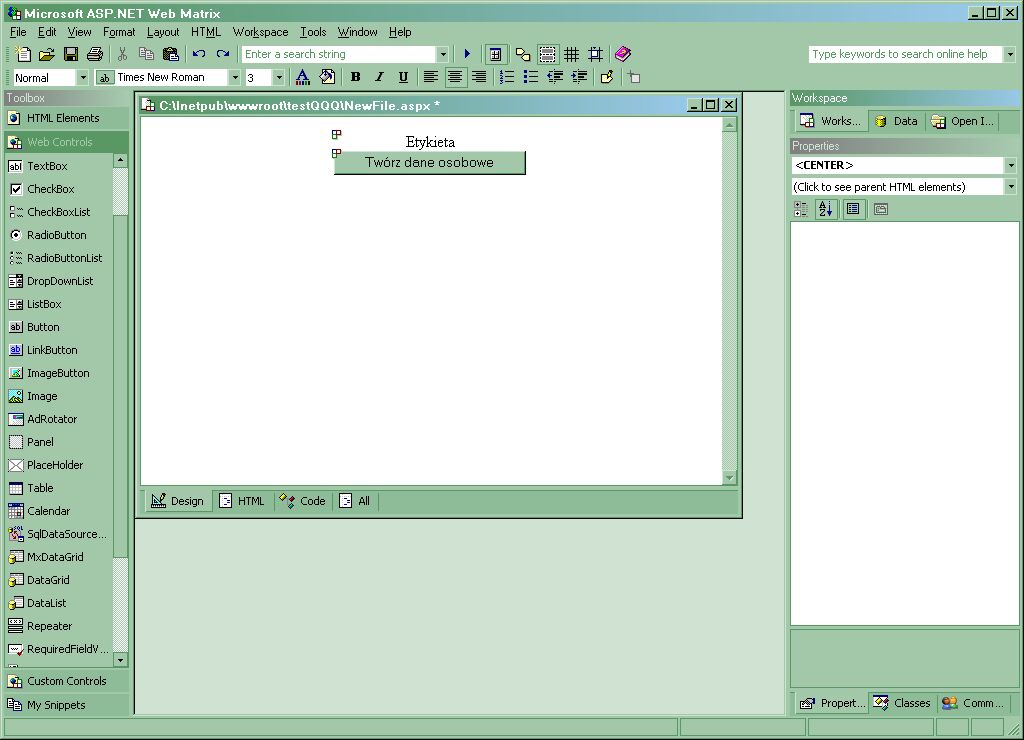
\includegraphics[width=0.75\textwidth]{./pic/asp02}
\caption{Microsoft ASP.NET WebMatrix w akcji}
\end{center}
\end{figure}
